%%%%%%%%%%%%%%%%%%%%%%%%%%%%%%%%%%%%%%%%%%%%%%%%%%%%%%%%%%%%%%%%%
%  _____       ______   ____									%
% |_   _|     |  ____|/ ____|  Institute of Embedded Systems	%
%   | |  _ __ | |__  | (___    Wireless Group					%
%   | | | '_ \|  __|  \___ \   Zuercher Hochschule Winterthur	%
%  _| |_| | | | |____ ____) |  (University of Applied Sciences)	%
% |_____|_| |_|______|_____/   8401 Winterthur, Switzerland		%
%																%
%%%%%%%%%%%%%%%%%%%%%%%%%%%%%%%%%%%%%%%%%%%%%%%%%%%%%%%%%%%%%%%%%

\chapter{Testbench}\label{chap.testen}
 \textit{Test Driven Development} bedeutet, dass vor oder parallel zur Entwicklung einer \textit{unit} (im Folgenden Block genannt) der \textit{unit-test} entwickelt wird\cite{Testdriven}. Beim textbasierten Testen stammen die Befehle aus einer Input-Datei, und die Ergebnisse werden in einer Datei abgelegt. 

\section{Device Under Test}\label{sec.testbench_DUT}
Das Device Under Test (DUT)  ist das midi interface. Das Ziel ist, dass das MIDI-Signal in den Block geführt wird und am Ausgang 10 Notenvektoren mit je 8 Notenbits und einem Bit, das besagt, ob die Note an oder ab ist.\\
\begin{figure}[H]
	\includegraphics[width=1\textwidth]{images/midi_interface/testbench_midiinterface.png}
	\caption{Blockschaltbild Device under Test}
	\label{fig.testbench}
\end{figure} 

Die \textit{testbench} wird mit Daten der Input-Datei gespiesen. Die Endversion der Input-Datei und der Testbericht liegen im Anhang \ref{chap.anhang_midi_input}. 
In den Unterkapiteln wird der Aufbau der Input-Datei, das Entwickeln der Test-Fälle, und die Umsetzung im VHDL-Code beschrieben.


\section{Struktur der Input-Datei}\label{sec.testbench_inputdatei} 

Die Test-Datei ist zeilenweise strukturiert.

\subsubsection{Verarbeitungsmodus} 
Jede Zeile beginnt mit dem Verabreitungsmodus. Bei der Input-Datei besteht der Verarbeitungsmodus aus fünf Buchstaben.

\begin{tabbing}
\hspace{4em} \= \hspace{2em} \= \hspace{2em} \=\kill
reset	\> 00 \> 00 \> \ldots{}\\
singl	\> 90 \> 27 \> \ldots{}\\
polyp	\> 71 \> 55 \> \ldots{}
\end{tabbing}

\subsubsection{Tokenstruktur} 

Nach dem Verarbeitungsmodus folgen die Daten. Jede Zeile hat gleichviele Datenpackete (Tokens). 
Die \textit{testbench} ortet jedem Datenpaket innerhalb der Zeile eine Bedeutung zu. Je nach Verarbeitungsmodus ist die Bedeutung der Token anders.

Die \textit{testbench midi interface} an den zwei MIDI Datentypen, die im Unterkapitel \ref{datenytpen} detailliert beschrieben sind. Die Tokestruktur leitet sich aus der Datenreihenfolge im \textit{polyphony mode} und im \textit{single mode} ab (siehe  \ref{note_modes}). In der nachfolgenden zwei Token-Beispielen bezieht sich die obere Zeile auf den \textit{polyphony mode} und die untere auf den \textit{single mode}.

In der \textit{testbench midi interface} haben Tokens folgende Bedeutung:


{
\renewcommand{\arraystretch}{1.0} % avoid the extra space between the rows
\begin{tabular}{@{}*{10}{l}@{}} % @{} removes the left and right margin around the table
mode\_p	& Note & Velocity	& Note & Velocity & Note & Velocity & Note & Velocity & Anzahl Noten \\
mode\_s	& Dummy & Status & Note & Status & Note & Status & Note & Dummy & Dummy
\end{tabular}
}

Dummy wird gesetzt, um die Verarbeitungsstruktur zu vereinfachen. Jeder Dummywert wird beim Einlesen verworfen.\\
 
\section{Aufstellen der Fehler}\label{sec.testbench_fehler} 

Die ersten Zeilen, sie sind ersetzt durch ausgefeiltere Datenstrukturen, hatten nur 3 Token und testeten die Grundfunktionen.\\

single mode note an/ab\\
singl 90 27\\ 
singl 90 27\\

polyphone note an/ab\\
polyp 71 55\\
polyp 71 00\\

Bei der Polyphonie ist notwendig, dass die einzelene Note unabhängig von den anderen Noten an oder ab bleibt. Die Test-Reihe wird deshalb auf 4 Noten ausgedehnt.


\subsection{Einzelne Noten testen}
 
\subsubsection{Testfälle}
Getestet sind auch Kombinationen unter den Fällen, die aus Übersichtlichkeit nicht alle aufgeschrieben werden.\\
\begin{itemize}
\item Einzelne Note an, Geschwindigkeits Byte folgt
\item Einzelne Note an, Geschwindigkeits Byte folgt nicht
\item Einzelne Note ab
\item Einzelne Note an, direkt nach Reset
\item Einzelne Note an, selbe Note nochmals an
\item Einzelne Note an, wenn in \textit{polyphonie mode}
\item Einzelne Note an, nach ungültigem status byte
\item Einzelne Note an, andere Note an, erste Note ab
\item Einzelne Note an, diverse andere Noten setzen, erst bei nächster Zeile erste Note ab
\end{itemize}

Zu jedem Testfall wird auf der nächsten Zeile das zu erwartende Resultat vorgegeben. Die testbench prüft die ausgegebene Notenwerte am Ausgang des midi interfaces mit den vorgegebenen Werten.

Beispielzeile\\
\rule{\textwidth}{0.4pt}\\
{
\renewcommand{\arraystretch}{1.0} % avoid the extra space between the rows
\begin{tabular*}{\textwidth}{@{}@{\extracolsep{\fill}}*{10}{l}@{}} % @{} removes the left and right margin around the table
singl & 55 & 90 & 27 & 80 & 27 & 90 & 05 & 00 & 00\\
check & 00 & 00 & 27 & 00 & 00 & 00 & 05 & 00 & 00\\
\end{tabular*}
}

Die Sequenz bedeutet Note 27 an (0x90), dann ab (0x80) der Note 27 und am Schluss an Note 05. \\
Überprüft (check) wird, ob am Ausgang die Noten 27 und 05 anliegen.\\
Im \textit{single mode} ist die Geschwindigkeit für das An- oder Abstellen der Note nicht relevant und wird deshalb nicht als Befehl eingelesen. Die \textit{testbench} hängt nach jeder Note einen Dummy-Geschwindigkeitswert von 0x55 an.

\subsubsection{Polyphonie testen }\label{polyphonitest}

\subsubsection{Testfälle}

In der Polyphony können mehrere Noten hintereinander an- und nur einzelne davon wieder abgestellt werden.

\begin{itemize}
\item Polyphoniestatus setzen, einzelne Note an
\item Polyphoniestatus setzen, mehrere Note an
\item Polyphoniestatus setzen, mehrere Note über mehrere Zeilen verteilt an
\item Polyphoniestatus setzen, Note an, die bereit in Register ist
\item Polyphoniestatus setzen, Note an, andere Note an, erste Note aus, dritte Note an
\item Polyphoniestatus setzen, dritte Note aus, erste Note an, erste Nte an
\item Polyphoniestatus setzen, singel Note an status setzen, Note ohne Geschwindigkeit senden
\item Polyphoniestatus setzen, falsches Statusbyte senden, Note an, Note aus,
\item Polyphoniestatus setzen, Reset, Note setzen
\item Polyphoniestatus setzen, 10 Noten an
\item Polyphoniestatus setzen, 10 Noten in Register, eine ist aus. Neue Note an senden
\end{itemize}

Beispielzeile\\
\rule{\textwidth}{0.4pt}\\
{
\renewcommand{\arraystretch}{1.0} % avoid the extra space between the rows
\begin{tabular*}{\textwidth}{@{}@{\extracolsep{\fill}}*{10}{l}@{}} % @{} removes the left and right margin around the table
polyp & 71 & 55 & 02 & 55 & 33 & 55 & 08 & 00 & 00\\
check & 71 & 00 & 02 & 00 & 33 & 00 & 00 & 00 & 03
\end{tabular*}
}

In der Sequenz wird die Note 71, dann die Noten 02 und 33. Danach wird die Note 08 abgestellt. Die \textit{testbench} prüft am Ausgang, ob die Noten 71, 02 und 33 an sind. 

Im Verarbeitungsmodus Polyphonie sendet die \textit{testbench}  das \textit{status byte} "10100000" (0xA0) 



\section{Code Testbench}\label{sec.code_testbench}
Die automatisierte Datenverarbeitung erzeugt viele Werte (10 Noten mit je 9 Werten). Um einzelne Bits effizient zu setzen oder zu überprüfen, wird der Code einem \textit{refactoring} unterzogen.

Im Gegensatz zum hardwarenahen Code der VHDL-Blocks, bei denen arrays und loop explizit vermieden wurden, baute die \textit{testbench} bewusst auf softwarenahe Strukturen auf.

\subsection{Erstellen eines Package}
\begin{itemize}
	\item Werte der \textit{status bytes} als Konstanten
	\item Ein- und Ausgänge als arrays
	\item Tokenstruktur als record
\end{itemize}

Bsp. Tokenstruktur

\begin{lstlisting}[language=vhdl]
-- define midi_data
type t_midi_data is record
    token_note : std_logic_vector(7 downto 0);
    token_attribut : std_logic_vector(7 downto 0);
    end record;

type t_midi_data_array is array (0 to 3) of t_midi_data;

-- define token structure
type t_token_line is record
    token_cmd : string(1 to 5);
    t_midi_data : t_midi_data_array;
    token_number : std_logic_vector(7 downto 0);
    end record;

-- array with note structure (input/output)
type t_note_array is array (0 to 9) of std_logic_vector(8 downto 0);
\end{lstlisting}


\subsection{Prozessoptimierung}

Um die einzelnen Bits in den arrays zu setzen, braucht es in der Ablaufstruktur Optimierungen.

\begin{itemize}
	\item loops iterieren durch die arrays
	\item Einleseprozess wird vom Verarbeitungsprozess getrennt
	\item Flags wie \lstinline|s_read_input_finished <= '1'| sichern das parallelle Datenverarbeiten
\end{itemize}

\section{Ergebnisse Simulation}\label{sec.ergebnisse_tests}
Die Ausgabe der Signale in die Output-Datei bezieht sich auf den Zustand am Ausgang des DUT. Damit auch die beiden internen Blöcke midi control und polyphonie out korrekt funktionieren werden die Signale überprüft. Auch das Verhalten in den Blöcken entspricht den erwarteten Signalverläufen.\\

\subsection{Block Midi Control}
Gemäss der \textit{fsm} durchläuft der \textit{single mode}  die Zustände idle, note\_s, velocity\_s und geht dann zurück  in den idle-Zustand. Das Signal s\_note\_on wechselt nach einem \textit{status byte} von (0x90) auf on und nach (0x80) auf ab.
\begin{figure}[H]
	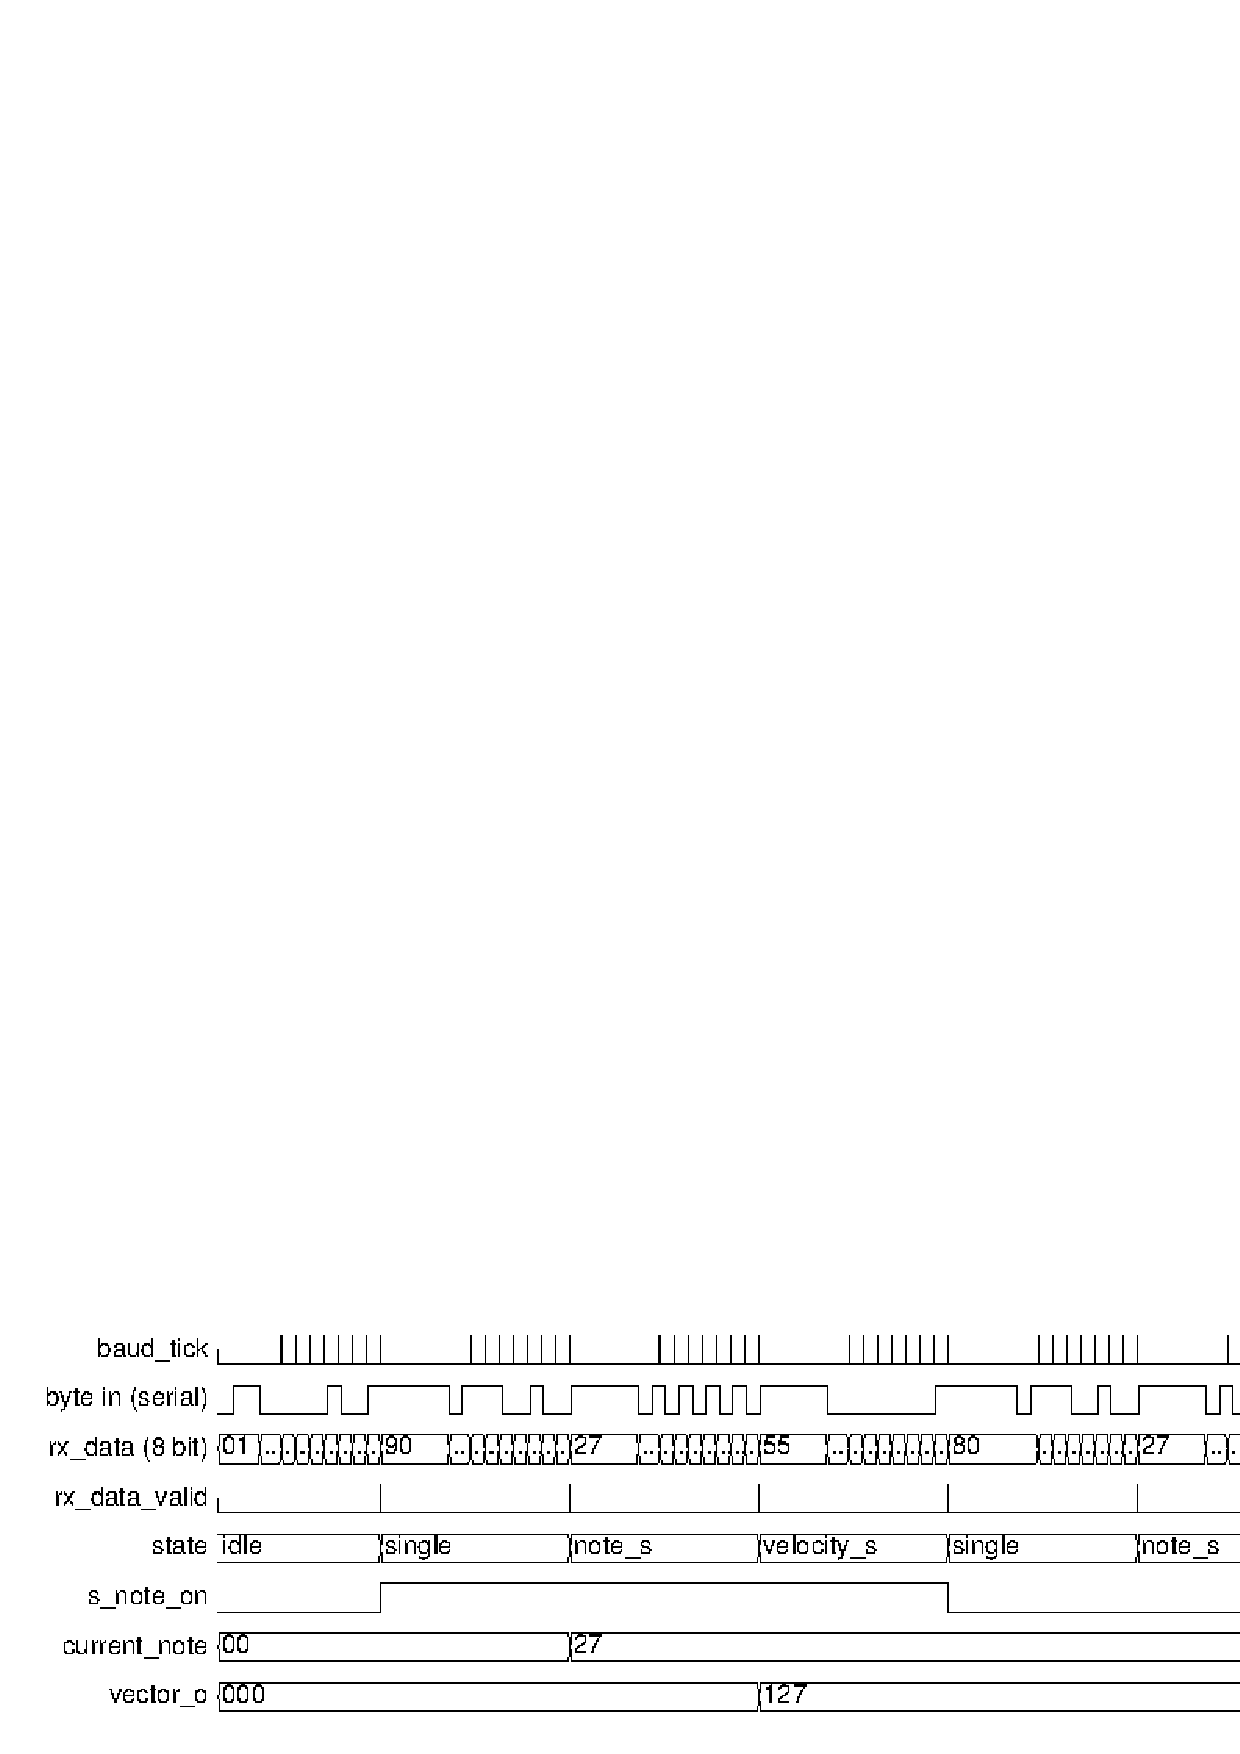
\includegraphics[width=1\textwidth]{images/midi_control/wave_single.png}
	\caption{Simulation Block Midi Control}
	\label{fig.test_midi:control_single}
\end{figure} 

Im \textit{polyphony mode} existieren die Zustände idle, note\_v, velocity\_v und verbleibt in diesem Zustand. Nur durch ein \textit{status byte} (oder ungültige \textit{data bytes}) wird der Zustand der Polyphonie verlassen.

\begin{figure}[H]
	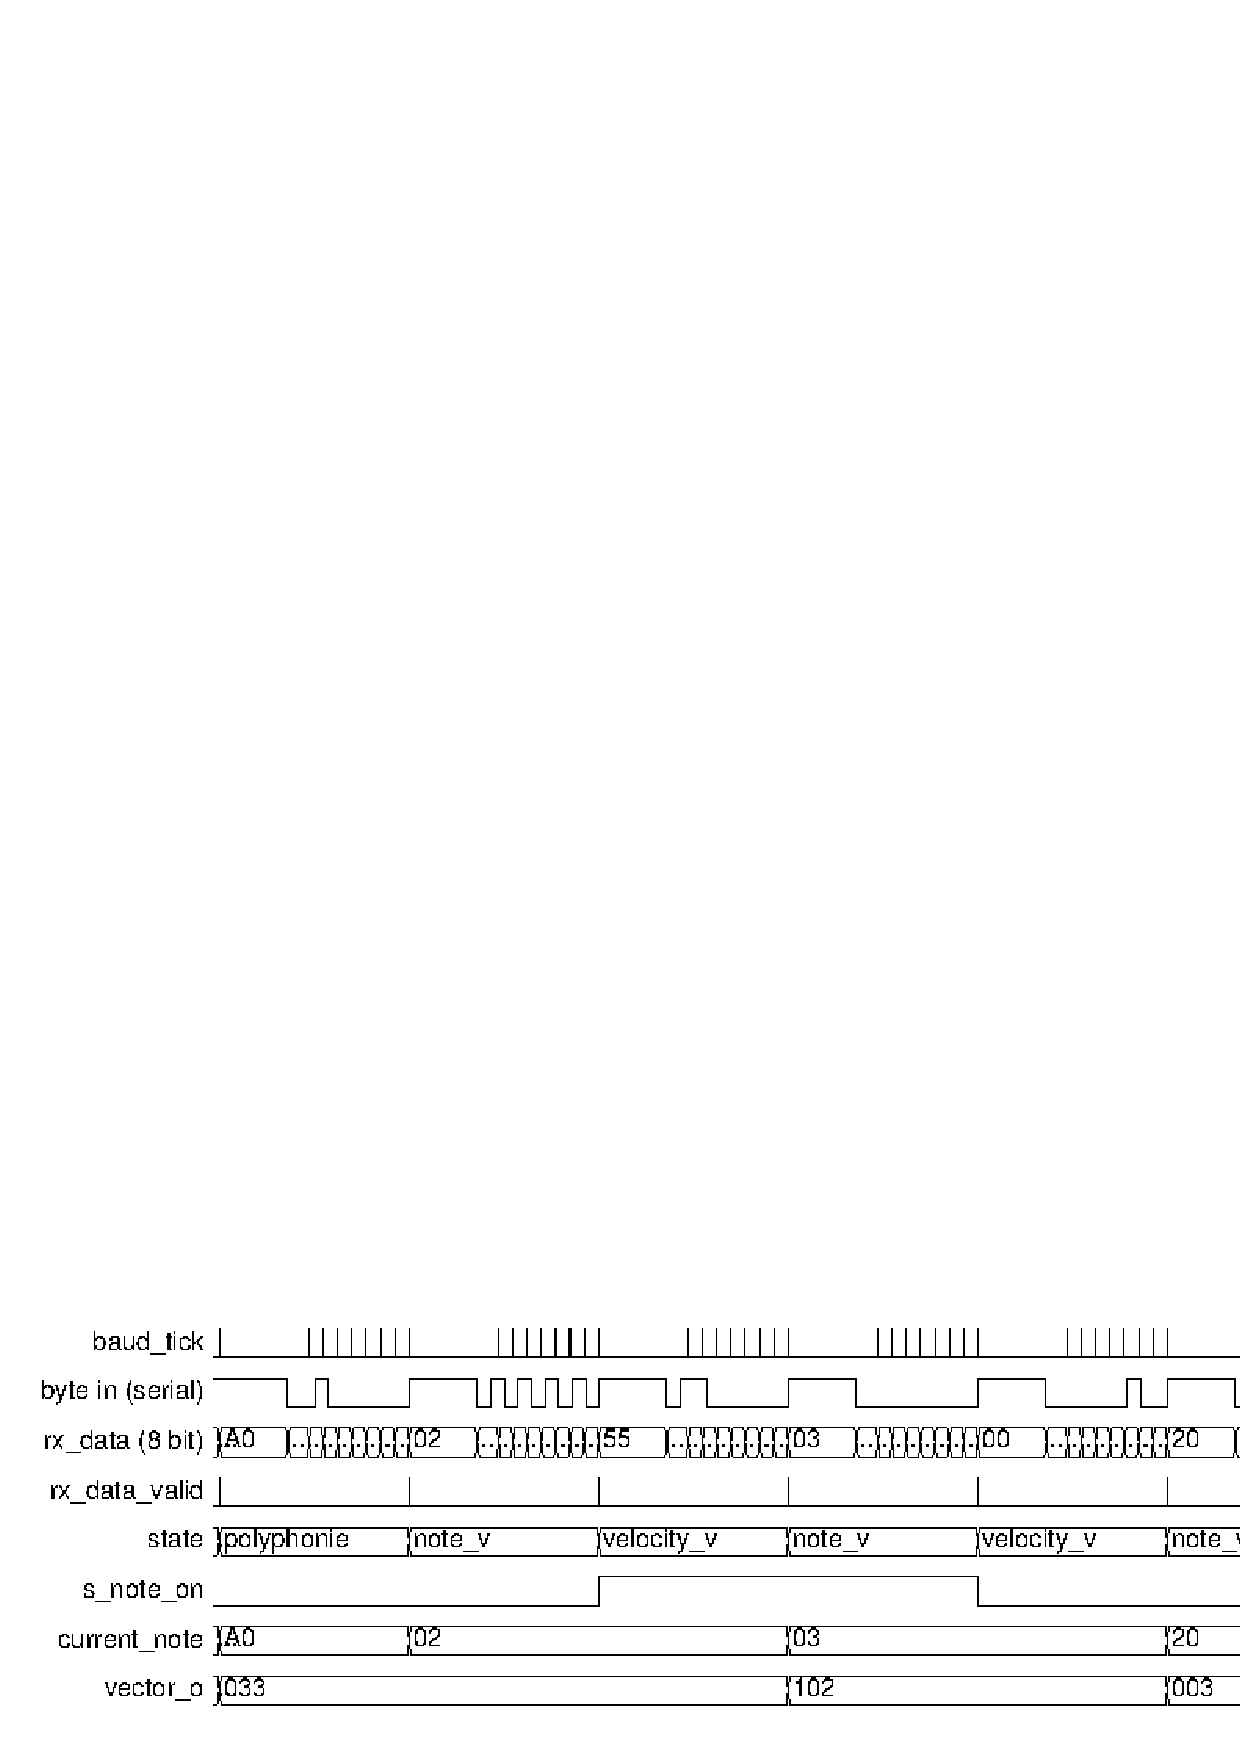
\includegraphics[width=1\textwidth]{images/midi_control/wave_polyphonie.png}
	\caption{Simulation Block Midi Control}
	\label{fig.test_midi:control}
\end{figure} 

\subsection{Block Polyphonie Out}
Kriterien in der Polyphonie out sind, dass jede neue Note auf den nächt freien Register-Platz gelegt wird. Zudem soll keine Note zwei Registerplätze belegen. Zudem soll, wenn alle Register-Plätze einen Notenwert haben, die neue Note an einen Registerplatz mit aktuell abgeschaltener Note besetzen.
Alle Kriterien sind erfüllt.\\

\begin{figure}[H]
	\includegraphics[width=1\textwidth]{images/midi_interface/tb_polyphonie.png}
	\caption{Simulation Block Polyphonie Out}
	\label{fig.test_polyphonie}
\end{figure} 

